\section{Exploración inicial: afluencia del Metro}\label{sec:exploracion}

La afluencia del Metro es la serie de movilidad \textbf{más larga y detallada} disponible: es
diaria, por estación, y cubre de 2010 a 2026. Se exploró primero para ilustrar el fenómeno que se
estudiará y los problemas de calidad que habrá que limpiar. El código está en el notebook
\archivo{notebooks/00_contexto_y_datasets.ipynb}.

\subsection{Descripción del archivo}
El recurso \enquote{Afluencia Diaria del Metro (Simple)} tiene \textbf{1,180,920 registros}, del
2010-01-01 al 2026-07-31. Cada registro corresponde a un día, una línea y una estación. No tiene
valores nulos (Tabla~\ref{tab:perfil_metro}).

\begin{table}[h]
\centering
\caption{Perfil de las columnas del archivo del Metro.}\label{tab:perfil_metro}
\small
\begin{tabular}{llrr}
\toprule
\textbf{Columna} & \textbf{Tipo} & \textbf{Nulos} & \textbf{Valores únicos}\\
\midrule
\archivo{fecha}     & fecha   & 0 & 6,056\\
\archivo{anio}      & entero  & 0 & 17\\
\archivo{mes}       & texto   & 0 & 12\\
\archivo{linea}     & texto   & 0 & 24\\
\archivo{estacion}  & texto   & 0 & 168\\
\archivo{afluencia} & entero  & 0 & 92,564\\
\bottomrule
\end{tabular}
\end{table}

\subsection{Problemas de calidad detectados}
\paragraph{1. Texto mal codificado (\emph{mojibake}).} El archivo se guardó con una codificación
incorrecta, por lo que las letras acentuadas aparecen alteradas. Esto afecta a \textbf{57 de los 168}
nombres de estación. Se reparó con la librería \archivo{ftfy}, y tras la reparación quedan
\textbf{165 estaciones} únicas, porque algunas variantes eran duplicados de la misma estación
(Tabla~\ref{tab:mojibake}).

\begin{table}[h]
\centering
\caption{Ejemplos de nombres de estación reparados.}\label{tab:mojibake}
\small
\begin{tabular}{ll}
\toprule
\textbf{Original} & \textbf{Reparado}\\
\midrule
\texttt{Isabel la Católica} & Isabel la Católica\\
\texttt{Pino Suárez} & Pino Suárez\\
\texttt{Gómez FarÃas} & Gómez Farías\\
\texttt{Pantitlán} & Pantitlán\\
\texttt{División del Norte} & División del Norte\\
\texttt{FerrerÃa/Arena Ciudad de México} & Ferrería/Arena Ciudad de México\\
\bottomrule
\end{tabular}
\end{table}

\paragraph{2. Nombres de línea inconsistentes.} La columna \archivo{linea} tiene 24 valores
distintos, pero el Metro tiene 12 líneas. Entre 2021 y 2023 el archivo escribe
\texttt{LÃnea 1} (con acento y mal codificado) y en los demás años \archivo{Linea 1}. Si no se
corrige, cada línea queda partida en dos series. Se normalizó a la forma \archivo{Línea N}.

\paragraph{3. Cierres de líneas.} La Línea~12 cerró tras el colapso del 3 de mayo de 2021, y la
Línea~1 cerró por su modernización a partir de julio de 2022. Estos cierres reducen la afluencia por
causas ajenas a la demanda, así que deben marcarse para no confundirlos con una falta de
recuperación (Tabla~\ref{tab:lineas}).

\subsection{Comportamiento de la serie}
La Figura~\ref{fig:metro} muestra la afluencia mensual con los periodos de análisis sombreados. Hay
dos choques visibles:
\begin{itemize}
  \item Uno \textbf{puntual}: el sismo del 19 de septiembre de 2017.
  \item Uno \textbf{prolongado}: la pandemia, con una caída abrupta en marzo--abril de 2020 y una
        recuperación lenta que todavía no está completa.
\end{itemize}

\begin{figure}[h]
\centering
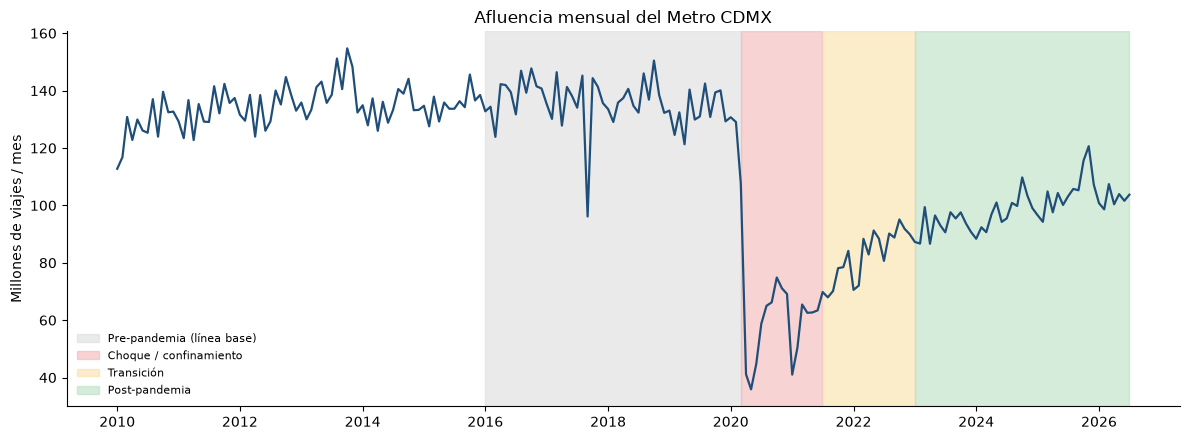
\includegraphics[width=\textwidth]{figuras/metro_mensual.png}
\caption[Afluencia mensual del Metro de la CDMX, 2010--2026]{Afluencia mensual del Metro de la CDMX, 2010--2026, con los periodos de análisis sombreados.
Fuente: elaboración propia con datos del STC Metro (Portal de Datos Abiertos de la CDMX).}
\label{fig:metro}
\end{figure}

\subsection{Caída y recuperación respecto a 2019}
Para medir la caída y la recuperación en términos relativos se construyó un índice con base
$2019 = 100$:
\[
  I_t = \frac{\text{afluencia}_t}{\overline{\text{afluencia}}_{2019}} \times 100
\]
donde $\overline{\text{afluencia}}_{2019}$ es el promedio mensual de 2019.

\begin{itemize}
  \item \textbf{Mes más bajo:} mayo de 2020, con $I = 27.0$, es decir, una \textbf{caída del 73\,\%}
        respecto a 2019. Esto respalda la hipótesis H1, que planteaba una caída mayor al 50\,\%.
  \item \textbf{Último mes disponible:} julio de 2026, con $I = 78.1$. La afluencia \textbf{aún no
        recupera} el nivel previo a la pandemia.
\end{itemize}

\begin{table}[h]
\centering
\caption{Índice promedio anual de afluencia del Metro ($2019 = 100$). *2026: enero a julio.}\label{tab:indice}
\small
\begin{tabular}{lccccccccccc}
\toprule
\textbf{Año} & 2016 & 2017 & 2018 & 2019 & 2020 & 2021 & 2022 & 2023 & 2024 & 2025 & 2026*\\
\midrule
\textbf{Índice} & 104.3 & 101.3 & 103.3 & 100.0 & 56.1 & 49.8 & 64.6 & 69.9 & 73.5 & 78.7 & 77.0\\
\bottomrule
\end{tabular}
\end{table}

\begin{table}[h]
\centering
\caption{Afluencia anual por línea (millones de viajes), con los nombres de línea ya normalizados.}\label{tab:lineas}
\small
\begin{tabular}{lrrrrrrr}
\toprule
\textbf{Línea} & 2019 & 2020 & 2021 & 2022 & 2023 & 2024 & 2025\\
\midrule
Línea 1  & 237.5 & 137.5 & 128.0 & 108.0 & 63.3  & 67.8  & 120.1\\
Línea 2  & 269.1 & 137.7 & 113.5 & 177.1 & 198.8 & 212.2 & 217.0\\
Línea 3  & 222.4 & 124.1 & 107.5 & 164.1 & 172.4 & 172.3 & 175.1\\
Línea 4  & 29.0  & 16.1  & 15.9  & 23.4  & 26.5  & 24.9  & 25.1\\
Línea 5  & 78.0  & 44.0  & 44.1  & 56.0  & 59.9  & 59.6  & 56.7\\
Línea 6  & 49.9  & 26.1  & 23.5  & 35.7  & 40.0  & 38.8  & 38.8\\
Línea 7  & 108.2 & 55.0  & 51.9  & 69.0  & 78.9  & 85.6  & 88.9\\
Línea 8  & 133.6 & 76.4  & 82.7  & 115.6 & 128.2 & 124.6 & 118.2\\
Línea 9  & 99.6  & 59.3  & 62.6  & 87.6  & 95.8  & 80.6  & 94.5\\
Línea 12 & 134.9 & 78.2  & 22.1  & 0.0   & 46.0  & 105.0 & 118.6\\
Línea A  & 79.9  & 52.0  & 54.8  & 72.9  & 75.7  & 71.7  & 77.1\\
Línea B  & 152.5 & 87.8  & 87.5  & 120.5 & 129.7 & 128.6 & 125.3\\
\bottomrule
\end{tabular}
\end{table}

\paragraph{Lectura preliminar.} En 2025, la afluencia total equivale al 78.7\,\% de la de 2019.
Si se excluyen las Líneas~1 y 12, afectadas por cierres, la proporción sube al 83.2\,\%. La Línea~1,
reabierta de forma parcial, apenas llega al 51\,\%. Aun sin los cierres, ninguna línea ha vuelto al
nivel de 2019: van del 73\,\% (Línea~5) al 96\,\% (Línea~A). Esto sugiere un efecto persistente de
la pandemia sobre la demanda, posiblemente por el teletrabajo (hipótesis H3). Al mismo tiempo,
confirma que el análisis de recuperación debe separar el efecto de la pandemia del efecto de los
cierres de infraestructura.
